\documentclass[main.tex]{subfiles}

\everymath{\displaystyle}
\begin{document}

\tiny

\begin{tabular}{cl}
	\toprule
	\\Partial Fraction Decomposition &
	$
	\begin{array}{lr}
		F(s) = \frac{N(s)}{D(s)}
		= \sum_{i=0}^n \sum_{k=1}^r \frac{K_{ik}}{(s+p_i)^k}
		\\\mathrm{K}_{ik} = \lim\limits_{s \to -p_i} \frac{1}{(r-k)!}
		\mathcal{D}^{r-k}[\frac{\mathrm{N}(s)}{\mathrm{D(s)}}(s-p_i)^r]
	\end{array}
	$
	\\\midrule
	\\Transfer Function &
	$ 
	\begin{array}{ll}
		L(c) = L(r)
		\\G(s) 
		= \frac{C(s)}{R(s)} 
		= \frac{\Lap{P_{dr}}}{\Lap{P_{dc}}}
		= \frac{\Lap{c(t)}}{\Lap{r(t)}}
	\end{array}
	$
	\\\midrule
	\\Electrical Analysis &
	\begin{tabular}{lc}
		Time Model & S-Model (Impedance)
		\\$i(t) = Rv(t)$ & $R$ 
		\\$i(t) = CD[v(t)] $ & $\frac{1}{Cs}$ 
		\\$v(t) = LD[i(t)]$ & $Ls$
	\end{tabular}
	\\\midrule
	\\Mechanical Analysis &
	\begin{tabular}{lcl}
		Time Model & S-Model (Impedance) &
		\\$f(t) = Kx(t)$ & $K$ & Spring
		\\$f(t) = \mathrm{f}_vD[x(t)]$ & $\mathrm{f}_vs$ & Damper
		\\$f(t) = MD^2[x(t)]$ & $Ms^2$ & Mass (Newton's 1st law)
	\end{tabular}
	\\\midrule
	\\Mechatronics Analysis &
	$
	G(s) = \frac{\theta(s)}{v(s)} 
	\approx \left. \frac{K}{s+a} \right| 
	K = \frac{K_t}{Ri(s)}, a = \frac{D_m+\frac{K_tK_b}{R}}{i(s)}
	$
	\\\midrule
	\\First Order Linear System &
	\begin{tabular}{lc}
		General Form     & $G(s) = \frac{K}{s+a}$
		\\ Time Constant & $T \approx \frac{1}{a}$
		\\ Rise Time     & $T_r \approx \frac{2.2}{a}$
		\\ Setting Time  & $T_s \approx \frac{4}{a}$
	\end{tabular}
	\\\midrule
	\\Second Order Linear System &
	\begin{tabular}{lc}
		General Form & $\frac{\omega_n^2}{s^2+2\omega_n\xi s+\omega_n^2}$
		\\ $\xi$      & $\left. \frac{\alpha}{2\omega_n} \right| \alpha =2\omega_n\xi$
		\\ $\omega_n$ & $\left. \sqrt{\beta} \right| \beta = \omega_n^2$
		\\ $T_p$      & $\frac{\pi}{\omega_n \sqrt{1-\xi^2}}$
		\\ $T_s$      & $\frac{4}{\omega_n\xi}$
		\\ $\%OS$     & $100\e^{-\xi\omega_n T_p}$
		\\ $T_r$      & 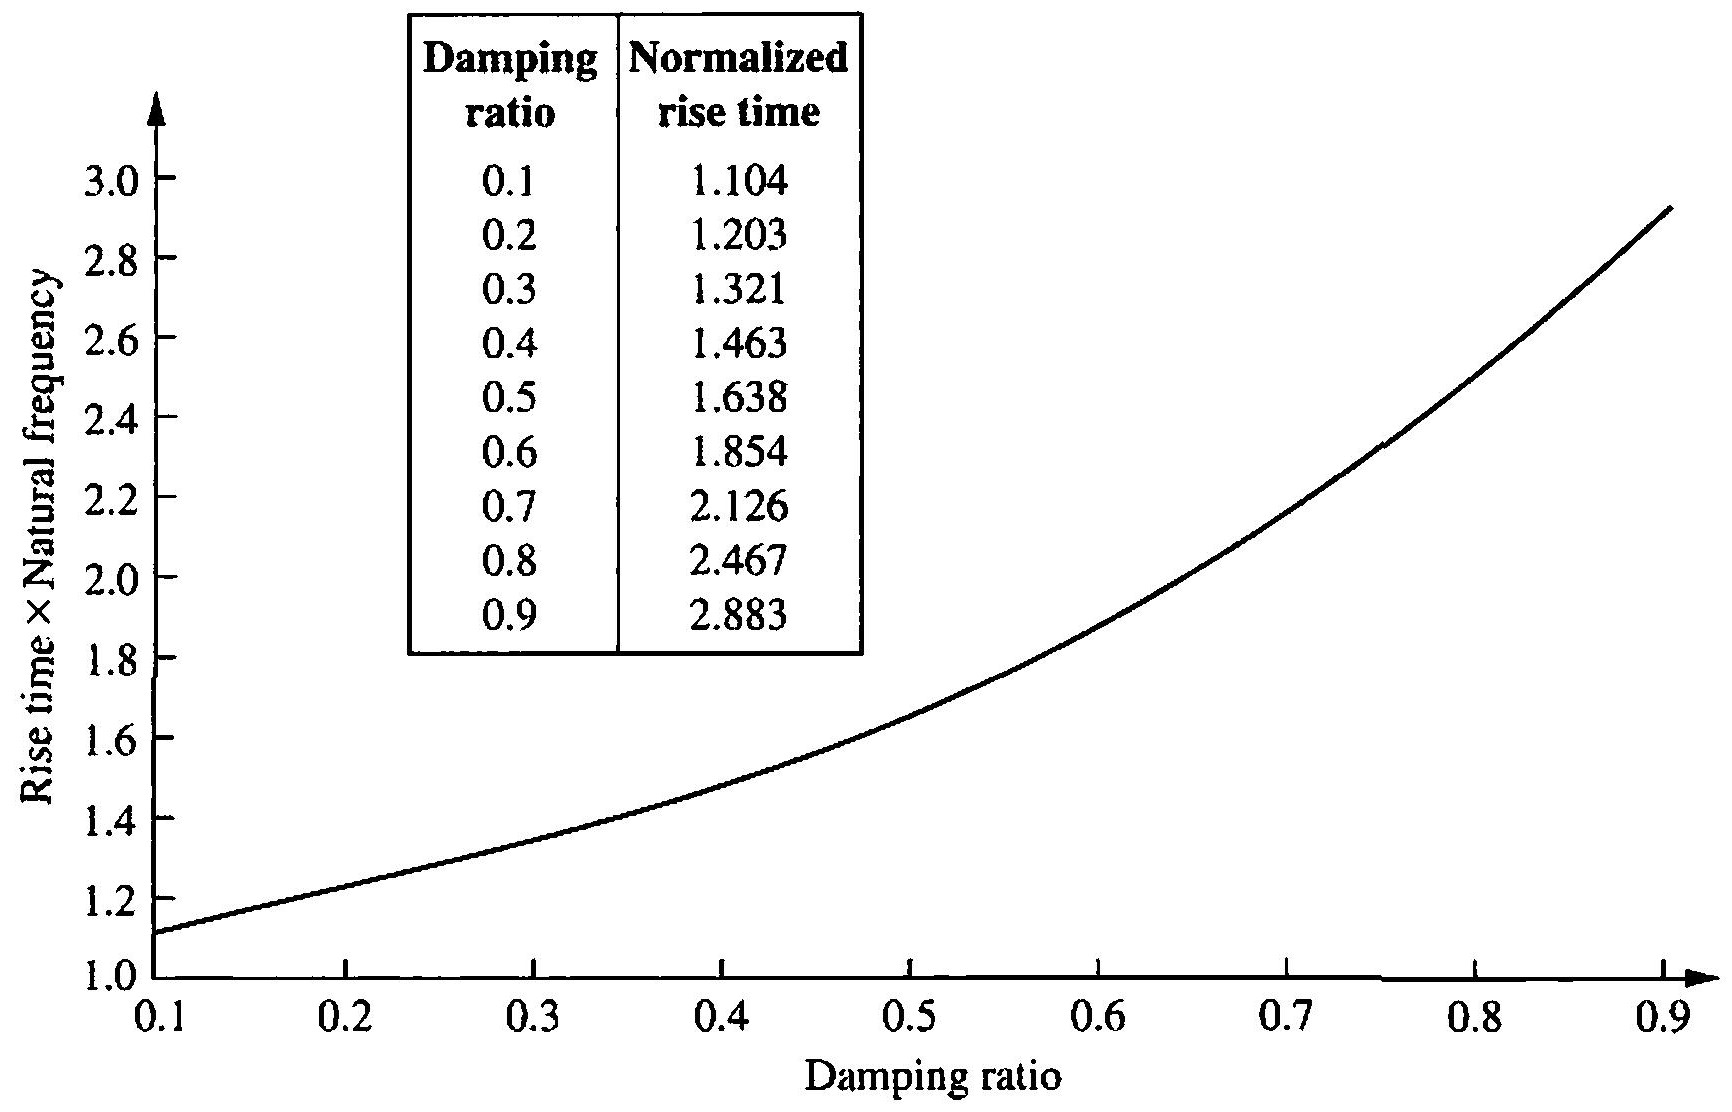
\includegraphics[width=2in]{riseTime}
	\end{tabular}
	\\\midrule
	\\Damping Characteristics &
	\begin{tabular}{lc}
		overdamped & $\xi > 1$
		\\critically damped & $\xi =1$
		\\under damped & $0 < \xi < 1$
		\\zero damping & $\xi = 0$
		\\unstable & $\xi < 0$
	\end{tabular}
	\\\midrule
	\\Steady State Error & 
	\begin{tabular}{lc}
		Assume $R(s) = \frac{\alpha}{s^{n+1}}$ & 
		$
		e_{ss} = 
		\begin{cases}
			0 & l > n
			\\ \frac{\alpha\prod{p_j}}{0^{n}\prod{p_j}+K\prod{z_i}}
			& l = n
			\\ \infty & l < n
		\end{cases}
		$		
		\\ Static Error Constants &
		$
		\lim_{s \to 0} 
		\begin{cases}
			K_p = G(S)
			\\K_d = sG(s)
			\\K_a = s^2G(s)
		\end{cases}
		$
		\\ Non-Unity Feedback &
		$G'(s) = \frac{G}{GH-G+1}$
	\end{tabular}
	\\\midrule
	\\Root Locus &
	\begin{tabular}{l}
		symetric about real axis
		\\ real segments lie where there are odd \# open loop zeros/poles.
		\\ asymtote: $\sigma_a = \frac{\sum^n P_i-\sum^m z_i}{n-m}$ $\theta_a = \frac{(2K+1)\pi}{n-m}$
		\\ break in/away: $\sum^n \frac{1}{x-p_i} = \sum^m \frac{1}{x-z_i}$ solve for $x$
		\\ $j\omega$ axis: 
		$1+G(j\omega)H(j\omega) = 0 \implies [A(\omega) = 0,jB(\omega)=0]$ solve for $\omega$
	\end{tabular}
	\\\midrule
	\\Stability &
	\begin{tabular}{ll}
		Only first col a zero & replace with $\epsilon$ and then keep going. Then
		find $lim_{\epsilon \to 0}.$
		\\Row of zeros & replace row with coefficients of derivitive of polynomial of
		previous row.
	\end{tabular}
	\\\midrule
	\\Notation &
	$
	\begin{array}{ll}
		L(y) = (P_{dy})y = \left(a_n(t)D^n + a_{n-1}(t)D^{n-1} + \cdots + a_1(t)D + a_0(t) \right)y
		\\ D^{n}y = \frac{\del{^ny}}{\del{t^n}}
	\end{array}
	$

	\\\bottomrule
\end{tabular}

\end{document}
